\documentclass[modern]{aastex62}

\usepackage{graphicx}
\usepackage{xcolor}
\usepackage{xspace}
\usepackage{amsmath}
\usepackage[sort&compress]{natbib}
\usepackage[hang,flushmargin]{footmisc}


% style tweaks
\newcommand{\acronym}[1]{{\small{#1}}}
\newcommand{\project}[1]{\textsl{#1}}
\newcommand{\code}[1]{{\texttt{#1}}}
\newcommand{\todo}[1]{\textcolor{red}{#1}}

% the following is stolen from Adrian Price-Whelan (github.com/adrn/latex-init):
\usepackage{hyperref}
\definecolor{niceblue}{rgb}{0.0, 0.4, 0.65}
\definecolor{linkcolor}{rgb}{0.02,0.35,0.55}
\definecolor{citecolor}{rgb}{0.4,0.4,0.4}
\hypersetup{colorlinks=true,linkcolor=linkcolor,citecolor=citecolor,
            filecolor=linkcolor,urlcolor=linkcolor}
\hypersetup{pageanchor=false}

% math
\newcommand{\Lone}[2]{\ensuremath{#1\| #2 \|^1_1}}
\newcommand{\Ltwo}[2]{\ensuremath{#1\| #2 \|^2_2}}

% astronomy
\newcommand{\teff}{\ensuremath{T_{\rm eff}}\xspace}
\newcommand{\logg}{\ensuremath{\log g}\xspace}
\newcommand{\feh}{\ensuremath{\mathrm{[Fe/H]}}\xspace}
\newcommand{\vt}{\ensuremath{v_t}\xspace}
\newcommand{\mh}{\ensuremath{\mathrm{[M/H]}}\xspace}
\newcommand{\xh}{\ensuremath{\mathrm{[X/H]}}\xspace}
\newcommand{\I}{\textsc{I}\xspace}
\newcommand{\II}{\textsc{II}\xspace}
\newcommand{\vsini}{\ensuremath{v \sin{i}}\xspace}
\newcommand{\gcm}{\ensuremath{\mathrm{g}~\mathrm{cm}^{-3}}\xspace}
\newcommand{\kms}{\ensuremath{\mathrm{km}~\mathrm{s}^{-1}}\xspace}
\newcommand{\ms}{\ensuremath{\mathrm{m}~\mathrm{s}^{-1}}\xspace}
\newcommand{\cms}{\ensuremath{\mathrm{cm}~\mathrm{s}^{-1}}\xspace}
\newcommand{\masyr}{\ensuremath{\mathrm{mas}~\mathrm{yr}^{-1}}\xspace}
\newcommand{\msun}{\ensuremath{\mathrm{M}_\odot}\xspace}
\newcommand{\ang}{\text{\normalfont\AA}\xspace}
\newcommand{\SNR}{\acronym{S/N}\xspace}


\newcommand{\TF}{\code{TensorFlow}\xspace}
\newcommand{\python}{\code{python}\xspace}
\newcommand{\wobble}{\code{wobble}\xspace}
\newcommand{\starry}{\code{\acronym{starry}}\xspace}
\newcommand{\HARPS}{\project{\acronym{HARPS}}\xspace}
\newcommand{\HIRES}{\project{\acronym{HIRES}}\xspace}
\newcommand{\RV}{\acronym{RV}\xspace}
\newcommand{\RVs}{\acronym{RV}s\xspace}
\newcommand{\EPRV}{\acronym{EPRV}\xspace}
\newcommand{\BERV}{\acronym{BERV}\xspace}
\newcommand{\PHOENIX}{\project{\acronym{PHOENIX}}\xspace}
\newcommand{\RM}{Rossiter-McLaughlin effect\xspace}
\newcommand{\LSF}{\acronym{LSF}\xspace}
\newcommand{\PCA}{\acronym{PCA}\xspace}




% stolen from Ben Pope:
\newcommand{\kepler}{\emph{Kepler}\xspace}
\newcommand{\hipparcos}{\emph{Hipparcos}\xspace}
\newcommand{\gaia}{\emph{Gaia}\xspace}
\newcommand{\ktwo}{\emph{K2}\xspace}

% misc shortcuts
\newcommand{\flatiron}{Flatiron Institute, Simons Foundation, 162 Fifth Ave, New York, NY 10010, USA}
\newcommand{\chicago}{Department of Astronomy and Astrophysics, University of
Chicago, 5640 S. Ellis Ave, Chicago, IL 60637, USA}
\newcommand{\Mdwarf}{Barnard's Star\xspace} % or should it be Barnard's star? or GJ 699?


\setlength{\parindent}{1.4em} % trust in Hogg
\begin{document}\sloppy\sloppypar\raggedbottom\frenchspacing % trust in Hogg

\shorttitle{\wobble}
\shortauthors{Bedell et al.}

\graphicspath{ {figures/} }
\DeclareGraphicsExtensions{.pdf,.eps,.png}

\title{\textsc{\wobble: a data-driven method for precision radial velocities}}

\author[0000-0001-9907-7742]{Megan Bedell}
\affiliation{\flatiron}

\author[0000-0003-2866-9403]{David W. Hogg}
\affiliation{\flatiron}
\affiliation{Center for Cosmology and Particle Physics, Department of Physics, New York University, 726 Broadway, New York, NY 10003, USA}
\affiliation{Center for Data Science, New York University, 60 Fifth Ave, New York, NY 10011, USA}
\affiliation{Max-Planck-Institut f\"ur Astronomie, K\"onigstuhl 17, D-69117 Heidelberg}

\author{Daniel Foreman-Mackey}
\affiliation{\flatiron}

\author[0000-0001-7516-8308]{Benjamin T. Montet}
\altaffiliation{Sagan Fellow}
\affiliation{\chicago}

\author{Rodrigo Luger}
\affiliation{\flatiron}

\correspondingauthor{Megan Bedell}
\email{E-mail: mbedell@flatironinstitute.org}

\begin{abstract}
% Context
Extreme-precision radial velocity (\EPRV) exoplanet surveys face considerable data analysis challenges in extracting maximally informative \RVs from spectra. 
Chief among these, particularly for the upcoming generation of red-optimized spectrographs targeting M dwarfs, is the presence of telluric absorption features, which cannot be perfectly modeled. 
Another major limitation on the achievable \RV precision is the need to adopt an imperfect stellar template against which to cross-correlate or otherwise match the observations. 
In both cases, the precision-limiting reliance on external information can be sidestepped using the data itself. 
%In both cases, the full data set of all observed spectra for a given target generally contains more complete information about the underlying 
%In both cases, using the full data set of all observed spectra for a given target will yield more precise constraints on the underlying spectra and their \RVs than a traditional analysis. %\todo{(reword this to be less controversial?)}
%Telluric absorption features in stellar spectra provide particular challenges to extreme-precision radial velocity (\EPRV) exoplanet surveys. 
%Large amplitude features are often masked in data analysis pipelines, reducing the number of observable spectral features which can be used to measure an \RV shift.
%Low-amplitude features that are hard to see even in high signal-to-noise spectra may be an important contributor to the overall \RV noise budget.
% Aims
Here we propose a data-driven method to simultaneously extract precise \RVs and infer the underlying stellar and telluric spectra using a simple linear model. 
We implement this method in \wobble, an open-source \python package which uses \TF in its first non-machine-learning application to astronomical data. 
In this work, we demonstrate the performance of \wobble on archival \HARPS spectra.
% Results
We recover the canonical exoplanet 51 Pegasi b, detect the secular \RV evolution of the M dwarf \Mdwarf, and retrieve the \RM for the Hot Jupiter HD 189733b. 
We also present extremely high-\SNR composite stellar spectra and detailed time-variable telluric spectra derived from these data. 
%This method may be of particular interest for future red-optimized spectrographs aiming to detect and characterize M dwarf host stars, where telluric features are considerable at wavelengths corresponding to the peak of the stellar spectral energy distribution.  
\end{abstract}

\section{Introduction}

Precise radial velocity (\RV) measurements are critical to the discovery and characterization of exoplanets. 
On order of one dozen dedicated spectrographs exist for the purpose of \RV planet-hunting, with at least as many more currently under construction \citep{Wright2017}. 
However, significant challenges exist in deriving precise \RV measurements from these spectra. 
%The current capabilities of extreme-precision radial velocity (\EPRV) instruments do not extend to the 10 \cms\ regime, 
%In this work, we present an open-source code for \RV\ determination. We use a highly flexible linear model to extract \RV s in a fully data-driven way. %Our method simultaneously models the stellar and telluric spectra.

One of the primary drivers of the \RV noise budget is the incomplete treatment of telluric features in the
Earth's atmosphere \citep{Halverson2016}. 
Often, particular sections of a spectrum that are likely to feature telluric features are identified before the velocity shift of the stellar spectrum is inferred. 
These regions are then removed from analysis, leaving only seemingly telluric-free regions to be analyzed \citep[e.g.][]{AngladaEscude2012}.

This method has two significant issues. 
The first is that removing sections of the spectrum can remove significant amounts of information about the star, lowering the precision at which we can measure the stellar radial velocity. 
Many of the regions of significant telluric absorption lie in the red-optical and near-infrared, where there are abundant narrow spectral features that can be used to improve \RV precision. 
This is especially true for M dwarfs, which peak in emitted energy at $\approx 1 \mu$m and have many narrow molecular absorption features in their photospheres \citep{Figueira2016}. 
Eliminating large chunks of these spectra will therefore significantly inhibit our ability to detect planets around M dwarfs through \RVs.

Secondly, not all telluric features are obvious. 
The Earth's atmosphere induces many small-amplitude features, often referred to as ``microtellurics,'' which are not obvious by eye but can affect the star's inferred \RV at the $\sim 1$ \ms level \citep{Cunha2014}. 
As the locations of these features are not known \textit{a priori} and may not even be apparent in stacked spectra of many observations, these spectral regions cannot be thrown out. 
Instead, alternative methods to account for these features as a part of the model must be developed and employed in order to mitigate the effect of the Earth's atmosphere on the measured stellar radial velocities.

One such approach is modeling the telluric spectrum using existing line databases like \acronym{HITRAN} \citep{HITRAN2016}. 
The telluric model may then be divided out from the observations, assuming the line spread function of the instrument is known \citep[e.g.][]{Seifahrt2010}. 
This method relies on existing physical knowledge about the Earth's atmosphere and can be fine-tuned using local observatory measurements of e.g. atmospheric water vapor content \citep{Baker2017}. 
However, line databases are incomplete even in significant absorption features when compared to actual observations and certainly do not include microtellurics, making them poorly suited for extreme precision RV applications \citep{Bertaux2014}.

Another option is the use of telluric standard observations: a spectrum of a rapidly rotating early-type star, which is virtually featureless due to extreme rotational line broadening, may be used as a telluric model and divided out. 
This approach has the advantage of naturally reproducing the instrumental line profile and current observing conditions if the standard star has a line-of-sight vector sufficiently close to the target and if both observations are taken close together in time. 
For these conditions to be true, though, requires a significant investment of observing time, which planet search programs often cannot afford. 
Additionally, artifacts may remain near strong telluric features due to the imperfect correction of unresolved features \citep{Bailey2007}.

An alternative approach is the simultaneous modeling of both telluric and spectral features from the data. 
As the Earth's motion around the barycenter of the solar system induces a Doppler shift considerably larger than both the motion of telluric features and the size of a single pixel on the detector, these two spectra can be disentangled.
This process is well-established in the analysis of binary star systems through the development of linear models \citep[e.g.][]{Simon1994} and in a Gaussian process framework \citep{Czekala2017}.
In these cases, both spectra are assumed to be unchanging in time, which is a reasonable approximation of a stellar spectrum but not necessarily of the telluric spectrum.
A more complicated model with time variability in the telluric spectrum may provide a more accurate fit. 
Work by \citet{Artigau2014} demonstrates that a Principle Component Analysis (\acronym{PCA}) approach is an effective way of parameterizing telluric spectral variability as a low-dimensional model derived from observational data. 
\citet{Artigau2014} use a library of telluric standard observations, which requires a significant investment of observing time to build up, but in principle such a data-driven model should be possible to derive from typical stellar observations provided enough epochs of data are available.

Just as imperfect telluric modeling can be a noise source in \EPRV analyses, the choice of stellar template can also be a major source of error. 
For stabilized, non-gas-cell \RV spectrographs, a standard approach has been to adopt a quasi-binary mask consisting of weighted top-hat functions at the expected locations of informative stellar absorption lines and cross-correlate this mask with the observed spectrum \citep[e.g.][]{Baranne1979, Pepe2002}. 
This approach is limited by the accuracy of the mask, and since most masks are built for a broad category of spectral type rather than customized for the individual star in question, it is unlikely that this techniques retrieve maximally precise \RVs. 
Deriving a custom spectral template by stacking all spectra iteratively as the \RVs are determined was shown to be a superior approach for stars with complex spectra by \citet{AngladaEscude2012}. 

Data analysis pipelines for absorption cell instruments have long used a stellar template that is customized to the star in question, although traditionally this template is a single observation taken for the purpose \citep[e.g.][]{Butler1996}. 
Higher quality templates can be derived iteratively from the data \citep{Sato2002, Gao2016}. 
\todo{(explain how this differs from what we'll do)}

\todo{(talk about lack of open-source code and difficulty of modifying \RV pipelines here?)}

Here we develop a linear data-driven model to infer the telluric and stellar spectra and calculate the stellar RV at each observed epoch. 
The telluric model component may vary with time in a low-dimensional manner, which is also inferred from the data. 
Our model requires no prior knowledge of the star or the Earth's atmosphere. 
As such, it does not yield absolute measurements of \RVs, only highly precise relative measurements between epochs.

In this work, we focus on the ultra-stabilized spectrograph case, i.e. a reliable instrumental calibration and no absorption cell. 
We also assume that multiple epochs of observations exist and that these epochs are spread out across the observing season(s). 
This assumption is necessary to enable the disentangling of telluric features from the stellar spectrum. 
In this sense our method is intended as a post-processing step, not a real-time data reduction service. 
However, the implementation that we present here is designed for flexibility and easy extensibility, and we discuss potential ways to overcome these limitations.

In Section \ref{s:methods}, we outline the model and its key underlying assumptions. 
We present an open-source implementation of this method in \python and \TF called \wobble. 
In Section \ref{s:results}, we demonstrate \wobble's capabilities by applying our method to \HARPS archival data for three target stars: the planet-hosting solar analog 51 Peg, the quiet M dwarf \Mdwarf, and the Hot Jupiter host HD 189733. 
We revisit many of the assumptions underlying \wobble in Section \ref{s:future} with a detailed look at the limitations of the current implementation. We outline potential ways of adapting \wobble\ for such cases as instruments with absorption cells, intrinsic time variability in the stellar spectrum, and lower-quality data. 
Finally, we conclude with a brief summary in Section \ref{s:conclusion}.

\section{Methods}
\label{s:methods}
\subsection{Model Assumptions}
\label{s:assumptions}

The model underpinning \wobble is designed to be flexible and easily extensible to a variety of situations. 
However, a few rigid assumptions are necessary, and we outline those here.

First, we assume that the wavelength calibration and spectral extraction of the instrument are perfect: that is, we begin at the stage of having 1D extracted spectra and corresponding wavelength grids in hand and we do not model any corrections to the wavelength solution.

We assume that the spectra can be modeled as the product of a finite number of components. 
For the cases shown in this work, two components are used: a stellar spectrum which is invariant in shape but may be Doppler-shifted, and a telluric spectrum which is fixed to the observatory rest frame but varies in shape. 
We choose to work in log(flux) space so that the data to be modeled are simply a sum of the component spectra.

For the case of the telluric component, whose spectrum is allowed to vary with time, we assume this spectral variability is low-dimensional. 
This assumption is physically motivated by the fact that a relatively small number of molecular species contribute to the telluric absorption spectrum. 
It is also needed in a practical sense, since every additional dimension over which the telluric spectrum can vary adds several thousand more free parameters to the model.

We assume that the stellar spectrum is invariant with time. 
This assumption will be revisited in Section \ref{s:future}. 

We assume that both the stellar and telluric spectra are approximately located at zero in logarithmic flux with small deviations due to absorption lines. 
As a result of this assumption, we are able to apply L1 and L2 regularization to the spectral templates. 
Regularization is a commonly used technique in machine learning, where large numbers of free parameters are standard. 
It is equivalent to applying a prior to the parameters which pushes them toward zero in the absence of strong evidence otherwise from the data. 
The strength of the regularization may be tuned to suit the data at hand through a cross-validation scheme: for example, the best-suited regularization in the bluest spectral orders may be much stronger for the telluric spectrum, where few features are present, than it is for the star, which generally has a dense forest of spectral lines. 
The exact implementation and validation of regularization in this model is further described in Section \ref{s:model-eqns}.

Aside from this regularization to push spectra to zero in the low-\SNR regime, the model makes no assumptions about the shape of the stellar or telluric spectra. 
We solve for spectral templates for each component as a series of pixels with no imposed correlations between them, meaning that the line spread function, covariances between lines arising from the same species, and other such physically expected correlations are not built into the model but must be learned in the process of optimizing. 
In addition to keeping this model simple, linear, and largely convex, this means that no physical knowledge about the object being observed is needed to extract its \RVs. 

For practical applications, the number of epochs $N$ must be large and span a significant fraction of the observing season. 
If the number of spectra is small or if all spectra are taken over a very small range of time (e.g. a single night), it will be nearly impossible to disentangle the components of the model from each other, as this process relies on the apparent Doppler shifting of the star(s) and Earth's atmosphere relative to each other. 
We will revisit this restriction in Section \ref{s:future}.

Finally, we assume that, when the stellar and telluric components are properly optimized, only Gaussian noise remains. 
This assumption will be revisited in Section \ref{s:future}.

\subsection{Model Specification}
\label{s:model-eqns}

We take the data to be the $M \times N$ matrix Y, where each entry $y_{m,n}$ is the observed logarithmic flux $\ln f$ for pixel $m$ of $M$ at epoch $n$ of $N$. 
We also have a corresponding $M \times N$ matrix of wavelength solutions. 
Again, the entries of this matrix are in logarithmic form ($\ln \lambda$). 
This choice makes the Doppler shift an additive term, considerably simplifying the math to follow.

We model each data column $y_n$ as the sum of the stellar and telluric spectra:
\begin{equation}
y_n = y_{\star, n} + y_{t, n} + noise.
\end{equation}

The stellar spectrum contribution is: 
\begin{equation}
y_{\star, n} = P(v_{obs, n}) \mu_{\star},
\end{equation}
where $P$ is an interpolation operator which applies a Doppler shift by velocity $v_n$ and $\mu_{\star}$ is a spectral template with length $M'$ corresponding to the length of an arbitrarily-chosen wavelength grid. 
Because we work in log-wavelength space, the Doppler shift due to velocity $v$ is simply an additive term:
\begin{equation}
 \ln \lambda(v) = \ln \lambda_{0} + \frac{1}{2} \ln \left(\frac{1 - v/c}{1 + v/c}\right).
\end{equation}
The $P$ operator adds this term to the $M'$-length wavelength grid for the template spectrum before linearly interpolating the template to the $M$-length data space.

The apparent stellar \RV, $v_{obs, n}$, is a sum of the star's actual velocity about its center of mass ($v_{\star, n}$) and the projected motion of the Earth about the Solar System barycenter (Barycentric Earth Radial Velocity or \BERV$_{n}$ ), the latter of which is known.

The telluric spectrum contribution is:
\begin{equation}
y_{t, n} =  A_n(\mu_{t} + W_{t} z_n)
\end{equation}
In addition to its mean spectrum $\mu_t$, the telluric component also takes a time-dependent component assembled from two variables: $W_t$, a matrix of ``basis vectors'' for the span of telluric spectral variations, is weighted by $z_n$ to form the spectral contribution at epoch $n$. 
$W$ has the shape $M' \times K$ and $z_n$ is a $K$-vector, where $K$ is the number of basis vectors used. 
For the purposes of this work we found good performance with $K$ set to 3, but this may vary for other applications. 
The net telluric spectrum (mean + time-variable components) is weighted by the air mass at the time of observation $A_n$, a known quantity.

We evaluate a log-likelihood for each epoch
\begin{equation}
\ln \mathcal{L}_n = \sum_{m} -0.5 (y_{m,n} - y'_{m,n})^T C_{m,n}^{-1} (y_{m,n}-y'_{m,n}),
\end{equation}
comparing our model $y'$ to the data $y$, with $C$ representing the covariance matrix of uncertainties on each data point.

The number of free parameters in this model is large: we must optimize every grid point in the mean spectral templates and telluric basis vectors along with the stellar \RV and the telluric basis weights for each epoch. 
We deal with potential over-fitting issues by applying L1 and L2 regularization to the spectral templates, as discussed in Section \ref{s:assumptions}. 

L1 normalization adds a term to the log-likelihood that takes the form:
$$ L1(p, \lambda) = \lambda \sum_{i} | p_{i} | ,$$
where $p$ is the vector of parameters to be normalized (in this case $\mu_{{\star}}$, $\mu_{{t}}$, or $W_{t}$) and $\lambda$ is the regularization amplitude.

Similarly, L2 normalization adds a term of the form:
$$ L2(p, \lambda) = \lambda \sum_{i} p_{i}^2 .$$

The effectiveness of the regularization depends sensitively on the value of $\lambda$ used: if $\lambda$ is too high, real features will be lost as the parameters are forced to zero, whereas setting $\lambda$ too low will make the regularization ineffective, leaving the model vulnerable to overfitting. 

We set regularization amplitudes for \wobble using a cross-validation scheme. 
In brief, we set aside 12.5\% of the total epochs as a validation set and, using some value of $\lambda$, run the model optimization on the remaining epochs (the training set). 
The resulting best-fit spectral templates and basis vectors are taken as fixed and the time-dependent terms only (\RVs and basis weights) are optimized for the validation epochs. 
The $\chi^2$ for the validation epochs can then be adopted as a goodness-of-fit measurement for the $\lambda$ value, and the procedure is repeated for different $\lambda$s to choose the best regularization amplitude. 
Because we have multiple regularization terms and multiple amplitudes to set, we begin by hand-setting all amplitudes to a reasonable starting guess and optimize each amplitude sequentially with cross-validation.

With regularization included, the final model likelihood is:
\begin{equation}
\begin{split}
\ln \mathcal{L} = & \sum_{n} \sum_{m} -0.5 (y_{m,n} - y'_{m,n})^T C_{m,n}^{-1} (y_{m,n}-y'_{m,n})  \\
 & + L1(\mu_{\star}, \lambda_{L1, \mu_{\star}}) + L2(\mu_{\star}, \lambda_{L2, \mu_{\star}}) + L1(\mu_{t},  \lambda_{L1, \mu_{t}}) + L2(\mu_{t},  \lambda_{L2, \mu_{t}}) \\
 & + L1(W_t, \lambda_{L1, W_t}) + L2(W_t, \lambda_{L1, W_t}) + L2(z_t, 1.0) ,
\end{split}
\end{equation}
where the regularization amplitude for the basis weights is arbitrarily set to 1.0 and all other regularization amplitudes $\lambda$ are set by grid searches using the above-described validation procedure. \todo{(HOGG: explain why regularization on basis weights is needed)} 

%In practice, the most effective regularization amplitudes can vary by orders of magnitude depending on the characteristics of the spectral region being used. 
%For instance, both $\lambda_{L1, \mu_{t}}$ and $\lambda_{L2, \mu_{t}}$ need to be much higher when the spectra in question span relatively blue wavelengths with few actual telluric features to fit than they do for the near-infrared wavelength regions with strong telluric features. 
%Similarly, the regularization amplitudes for the star tend to be higher for the G dwarf than they are for the M dwarf, which has far more absorption features in its spectra. 
%Setting the regularization amplitudes is therefore a crucial first step when applying the \wobble model to data.


\subsection{Optimizing the Model}
\label{s:optimizing}

As an initial guess, we set the star to be stationary, e.g. $v_{obs} = v_{BERV}$ at all epochs. 
We may then initialize the stellar spectrum $\mu_{\star}$ by Doppler-shifting the data and calculating the median flux across \BERV-corrected spectra in bins at each model wavelength $\lambda'$. 
The telluric template is initialized similarly by using the residuals after the stellar contribution has been removed, again binning in model wavelength (this time without applying any Doppler shift to the spectra) and taking the median values of each bin. 
Finally, we initialize the telluric spectrum's basis vectors $W_t$ and weights $z_t$ by performing Principal Component Analysis (\acronym{PCA}) on the residuals after both the stellar spectrum and the mean telluric spectrum have been removed. 
The $K$ highest eigenweights and their corresponding eigenvectors are taken as the basis weights and vectors. 

Once all parameters are initialized, we optimize them iteratively. 
The likelihood function is maximized first by varying the stellar and telluric templates (including the telluric basis vectors). 
This step is a convex optimization, meaning that a global optimum for the template parameters should be reached under the condition of fixed time-dependent variables. 
Next, the templates are held fixed and the time-dependent parameters (stellar \RVs and telluric basis weights) are varied to maximize the likelihood function again. 
\todo{(HOGG: how could this be made convex too?)}
We repeat this procedure, optimizing spectra and time-dependent parameters in turn, until the likelihood appears to converge, typically within 100 iterations.

The inverse variance uncertainty on the parameters is calculated as the Hessian, or the second derivative of the likelihood with respect to each parameter. \todo{(DFM: help me rephrase if needed?)}

\subsection{Combining Spectral Orders}
\label{s:combining-orders}

Most \EPRV instruments are echelle spectrographs spanning many orders. 
These orders are often treated as independent spectra when extracting \RVs, and the \RVs for each order are then combined in some manner to get a final time series. 

We follow this precedent and optimize the \wobble model individually for each order. 
While some \RV precision gain may be possible by inferring a global Doppler shift from all orders simultaneously, it is not clear that the gain would be worth the added computational expense, so we leave this for future work. 

After obtaining an $N$-epoch set of observed stellar \RVs from each of the $R$ spectral orders, we combine them by modeling each \RV $v_{n,r}$ as a combination of time-dependent stellar \RV, order-dependent \RV offset, and a Gaussian noise term:
\begin{equation}
v_{n,r} = v_n + v_r + \mathcal{N}(0,\,\sigma_{n,r}^{2} + \delta_r^2 )\,,
\end{equation}
where $v_n$ and $v_r$ are the characteristic \RVs at epoch $n$ and order $r$, $\sigma_{n,r}$ is the estimated measurement uncertainty on $v_{n,r}$, and $\delta_r$ is an additional jitter term specific to order $r$. 

\todo{(To do: fill in details: prior on $<v_r>$, optimization over $\delta_r$.)}

\subsection{Implementation}
\label{s:implementation}

The above-described model can be implemented in a variety of ways. We chose to build our code, \wobble, in \code{python} using \TF. 
\TF is a \todo{DFM: [blah blah technical blah]}. 
While it has primarily been used in machine-learning contexts in the astronomical literature \todo{(cite)}, its auto-differentiation and fast linear algebra capabilities make it valuable for this application as well. 
The necessary optimizations over many parameters can be performed with high efficiency by \TF: the below-described analysis of 91 spectra of 51 Peg runs in \todo{30} minutes on a standard Mac desktop.

Our code made open-source under the \acronym{MIT} license and is publicly available on GitHub.\footnote{\url{https://www.github.com/megbedell/wobble}}



\section{Application to \HARPS Data}
\label{s:results}

For the purposes of this work, we chose to test the performance of \wobble on archival spectra from the High Accuracy Radial Velocity Planet Searcher (\HARPS) spectrograph \citep{Mayor2003}. 
\HARPS has operated continuously since 2003 and as such has an extensive catalog of publicly available data. 
Furthermore, its excellent instrumental stability and careful calibration make the data ideally suited to our method, which relies on having an accurate wavelength solution for every spectrum. 

All data were obtained from the \acronym{ESO} public data archive in the form of ``\code{e2ds}'' spectra. 
These data are blocks of 72 order by 4096 pixel extracted 1D spectra. 
The airmass of the observation and the calculated \BERV are both provided in the \acronym{FITS} header of the spectral data file. 
We obtained wavelength solutions for each spectrum from the dedicated \HARPS calibration archive, also maintained by \acronym{ESO}. 
\todo{Uncertainty estimates for each pixel were calculated as... [HOGG, help me fill this in - relation to \SNR and conversion to log]}

Before running the above-described model optimization on the data, we first mask out any unreliably measured spectral regions and do a continuum normalization on each spectrum. 
This masking is done by setting the inverse variance on the masked data point to zero, effectively removing it from the fit. 
In brief, we mask pixels whose extracted flux is below zero as well as regions at the edges of the spectral orders where the local \SNR falls below 5. 
After masking these data, we convert the flux to log space and continuum normalize by fitting a polynomial to an asymmetrically clipped subset of the data. 

\todo{The final stellar \RV retrieved by \wobble is corrected for intra-night drift in the wavelength solution by subtracting off a drift term specified in the data header, consistent with the standard \HARPS pipeline.}

Below we describe the results of applying this procedure and optimizing the \wobble model using \HARPS data for stars of different types: a G dwarf with a known planet, an \RV-quiet M dwarf, and an early-K dwarf undergoing a planetary transit event.

\subsection{51 Pegasi}

For \wobble's first test, we chose the first known exoplanet host: 51 Pegasi. 
This target is a Sun-like star hosting a planet with an orbital period of 4 days and a mass of 0.5 Jupiter masses \citep{Mayor1995}. 
Its canonical status as the first exoplanet discovered means that large amounts of data exist for this system. 
In particular, archival \HARPS data exist mainly from efforts to observe reflected-light spectra of the planet \citep{Martins2015}. 

We ran \wobble on these archival data to test its performance on recovering a planetary signal with well-known orbital characteristics.\footnote{Based on data obtained from the ESO Science Archive Facility under request numbers mbedell329968 and mbedell331551.} 
The 91 publicly available spectra in the \HARPS archive are largely concentrated on a few nights of intensive observing, but these nights are sufficiently spread out throughout the year for a wide enough range in \BERV to disentangle the stellar and telluric spectra.

Despite the sparse phase coverage available across the planetary orbit, we recover a signal at the correct period and semi-amplitude in the \RVs (Figure \ref{fig:51peg_planet}). \todo{(numbers here, address the structure in residuals)}

Fits to an individual spectrum are shown in Figure \ref{fig:51peg_spectrum}. 
We emphasize that no \textit{a priori} information on e.g. expected spectral line positions and depths were used. 
The current realization of the \wobble algorithm treats each pixel of the template spectra as independent and has no line shape parameterization included. 
Nevertheless, the optimized stellar templates clearly reproduce the expected appearance of the spectra in a variety of regimes, from a crowded-line region to a sparser, continuum-dominated region to an extremely strong absorption line like the H$\alpha$ feature.

\begin{figure}
\centering
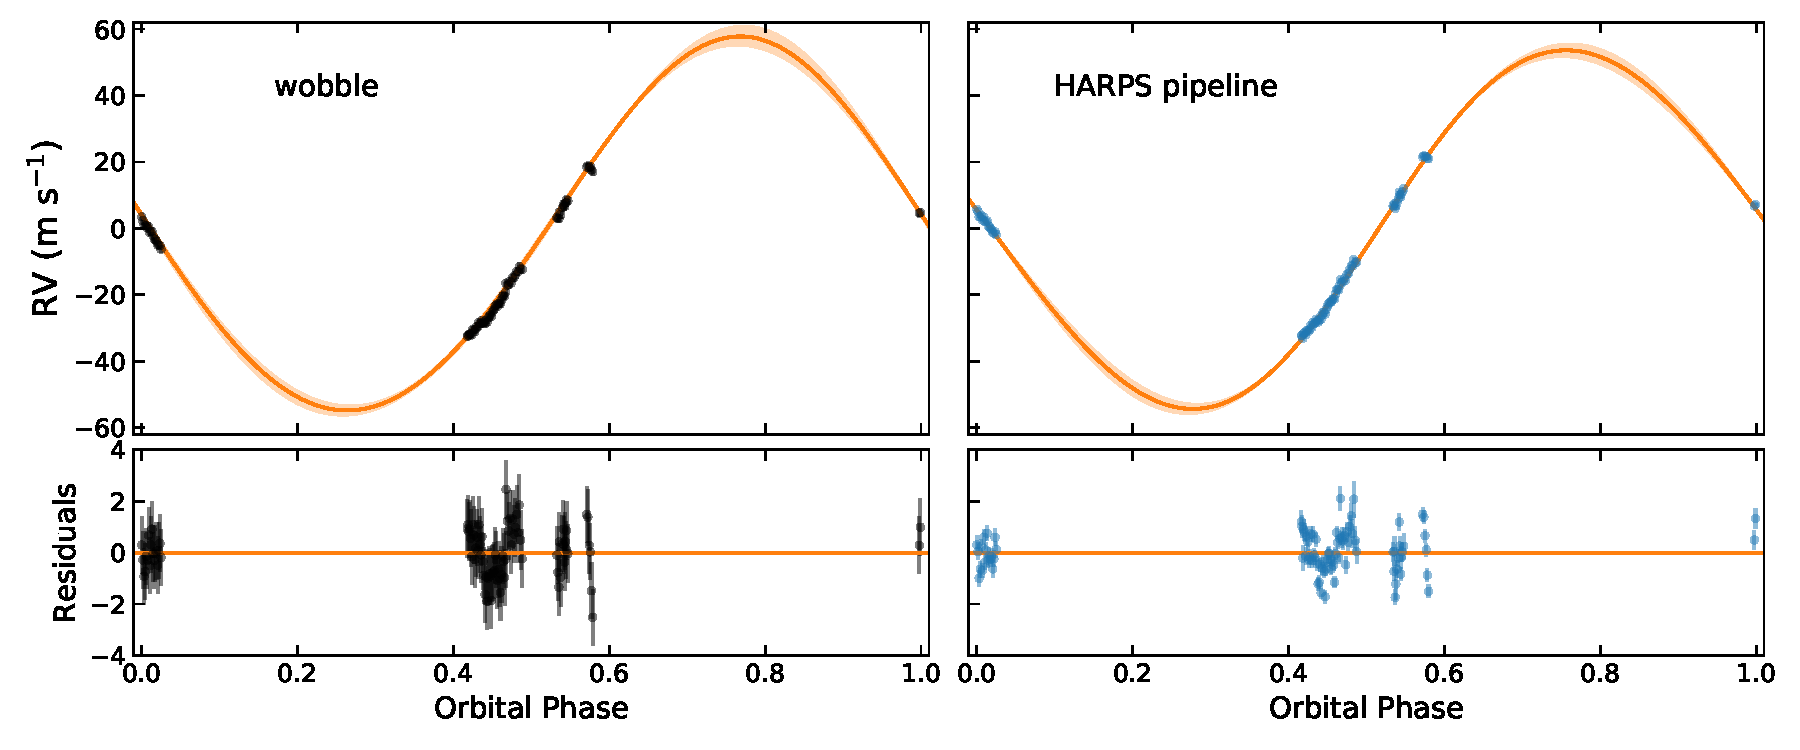
\includegraphics[width=4in]{51peg_planet}
\caption{Phased orbit of the Hot Jupiter 51 Peg b as recovered in the \wobble\ \RVs. While the phase coverage of \HARPS observations is sparse, we nonetheless recover orbital parameters consistent with those found by other \RV campaigns \todo{(add numbers)}.  \todo{check on: The subtle trends seen near secondary eclipse (phase 0.75) are suggestive of contributions by reflected light from the planetary dayside.}}
\label{fig:51peg_planet}
\end{figure}

\begin{figure}
\centering
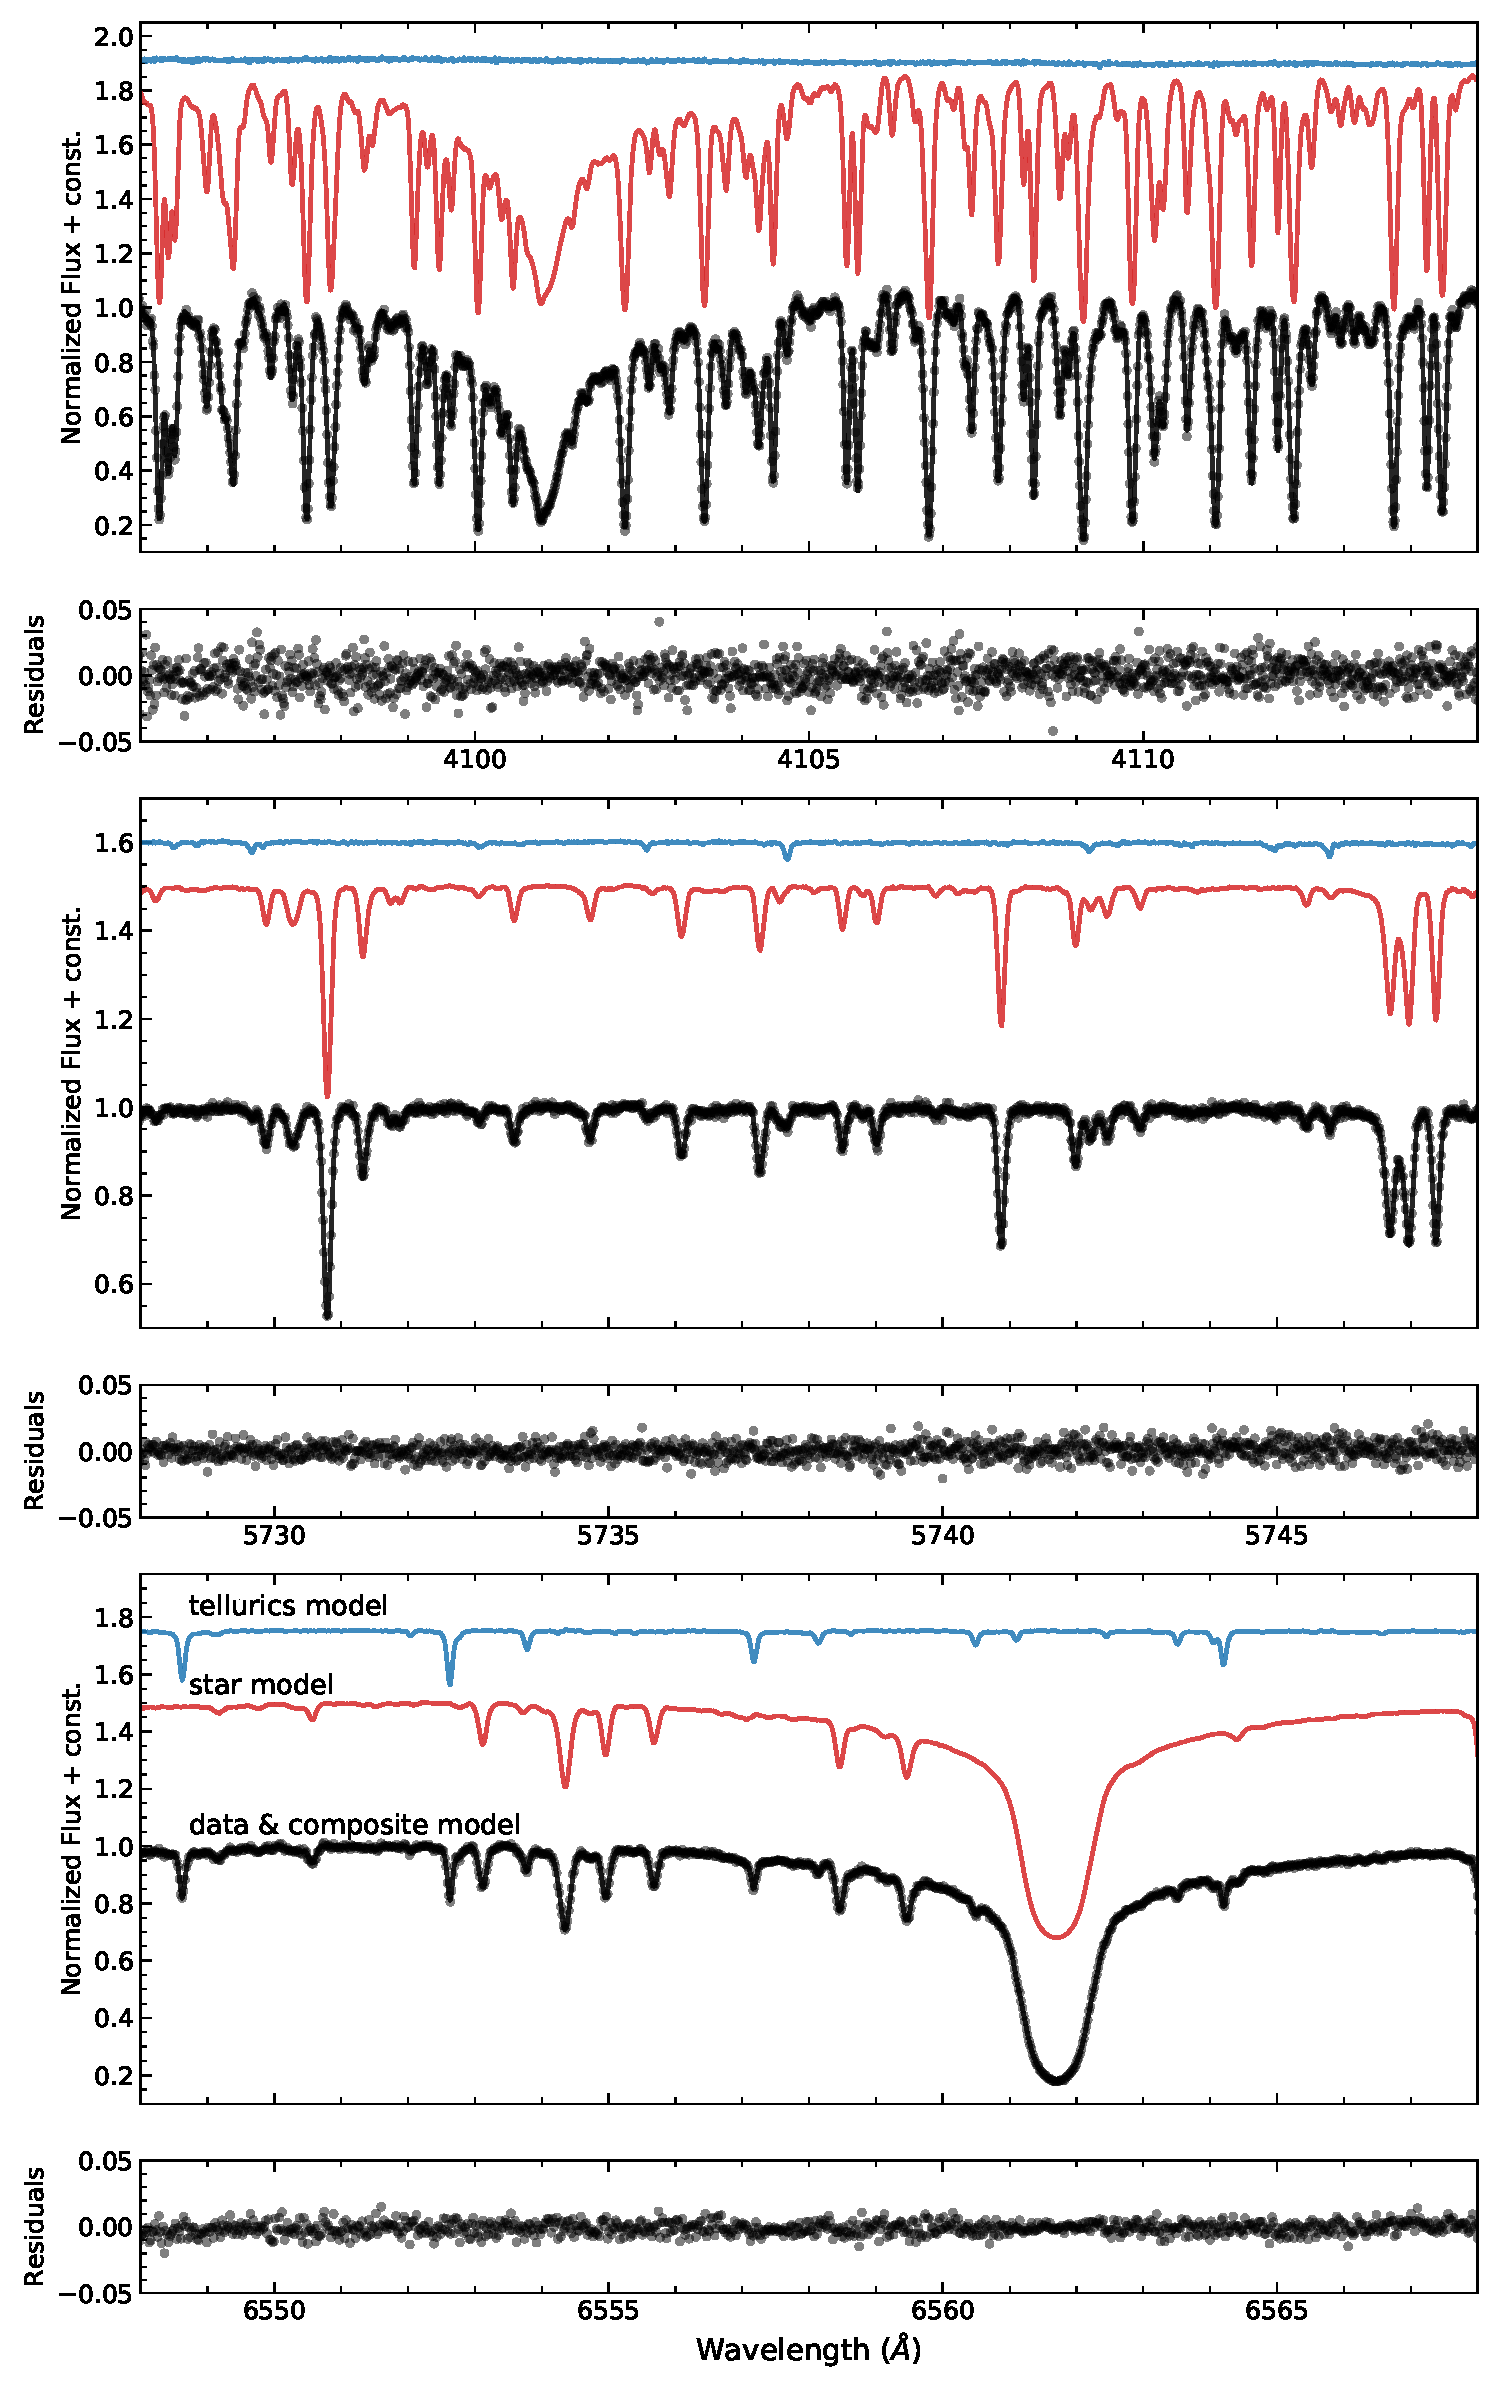
\includegraphics[width=5.3in]{51peg_multispectrum}
\caption{Three example echelle orders at a randomly chosen epoch from the \HARPS observations of 51 Pegasi. Data are shown as dark circles, while the \wobble predictions for the stellar and telluric spectral contributions at this epoch are red and blue lines, respectively. Even in the presence of a strong stellar absorption feature such as the H$\alpha$ line (seen at 6561.5 \ang due to the star's Doppler shift at the plotted epoch), small telluric features are clearly recovered. Residuals after subtracting both star and telluric models are shown below each spectrum.}
\label{fig:51peg_spectrum}
\end{figure}

\subsection{\Mdwarf}
\label{s:Mdwarf}

Next, we tested \wobble with 306 epochs of \Mdwarf spectra.\footnote{Based on data obtained from the ESO Science Archive Facility under request numbers mbedell359445 and mbedell359501.} 
\todo{(say brief things about data quality - it's low \SNR)}

\Mdwarf is one of the nearest stars to us at a distance of less than 2 parsecs. 
It is also the star with the highest known proper motion. 
Its trajectory translates to a projected secular change in \RV of approximately 4.5 $\mathrm{m}~\mathrm{s}^{-1}~\mathrm{yr}^{-1}$ \citep{Kurster2003}. 
This trend has been observed in some data sets, including long-term \HARPS and \acronym{HIRES} observations, although \acronym{UVES} \RVs were inconsistent with the predicted linear slope \citep{Kurster2003, Bonfils2013, Choi2013, Montet2014}. 
No planets have been found around \Mdwarf to date despite considerable amounts of \RV monitoring and little stellar activity has been observed, making it a good quiet star test case for \wobble. 

\begin{figure}
\centering
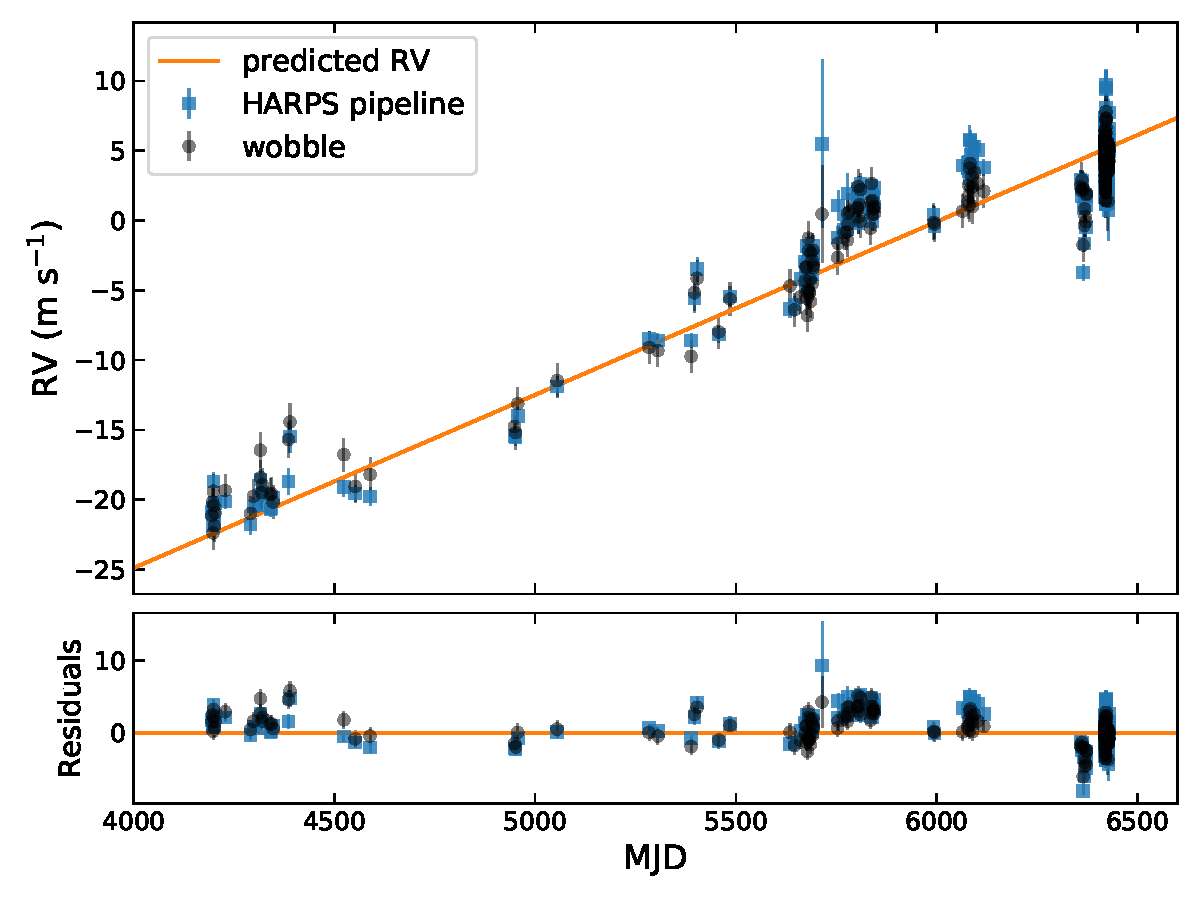
\includegraphics[width=5in]{barnards_rvs}
\caption{Radial velocity measurements for \Mdwarf from \wobble (black) and from the standard \HARPS pipeline (red). The median \RV has been subtracted from each data set. The predicted secular change in \RV due to \Mdwarf's projected motion, calculated using \gaia properties, is shown as a solid blue line (top panel). Residuals away from the predicted trend are plotted in the lower panel. \todo{(TO DO: add error bars)}}
\label{fig:barnards_rvs}
\end{figure}

The \RVs found by \wobble are in excellent agreement with the predicted secular motion (Figure \ref{fig:barnards_rvs}). 
Using \gaia parallax and proper motion measurements and following the calculations outlined in \citet{Kurster2003}, we find a secular trend with a slope of 4.53 $\mathrm{m}~\mathrm{s}^{-1}~\mathrm{yr}^{-1}$, deviating from this linearity by less than 1 $\mathrm{cm}~\mathrm{s}^{-1}~\mathrm{yr}^{-2}$ during the decade of \HARPS observations \citep{gaia2016, gaia2018}. 

After subtracting the \RVs as predicted by the equations of motion at each epoch, the residuals have low dispersion, as expected for a quiet star with no known planets. 
The \acronym{RMS} scatter among \wobble\ \RVs is 2.0 \ms. 
This compares favorably to the scatter of 2.5 \ms among \RVs produced by the standard closed-source \HARPS pipeline, although we note that many of the residuals have similar non-zero values in both independently produced RV estimates. 
It is possible that these deviations are a real physical effect in the stellar spectrum, but we caution that approximately \ms-level errors are likely being introduced by the barycentric correction. 
Currently we assume that the \BERV provided by the native \HARPS pipeline is correct, but this will not hold true if the sky coordinates entered by the observer deviate from the actual on-sky location of the target. 
This is especially likely to be the case for high proper motion targets like \Mdwarf. 
Indeed, we do note a strong peak at year-long periods in a Lomb-Scargle periodogram of the residual \RVs. 
Thus the \RV scatter derived in this work is only an approximate upper limit on the true precision achievable by \wobble. \todo{(TO DO: recalculate \BERV ourselves)}

Testing \wobble on the \Mdwarf data allows us to evaluate its performance in a significantly different regime: the mid-M dwarf spectra are far denser in spectral features than a Sun-like star, and individual observations are at a much lower \SNR than the 51 Peg observations used above, although the total number of spectra is greater. 
The resulting spectral fit is shown in Figure \ref{fig:barnards_spectrum}.

\begin{figure}
\centering
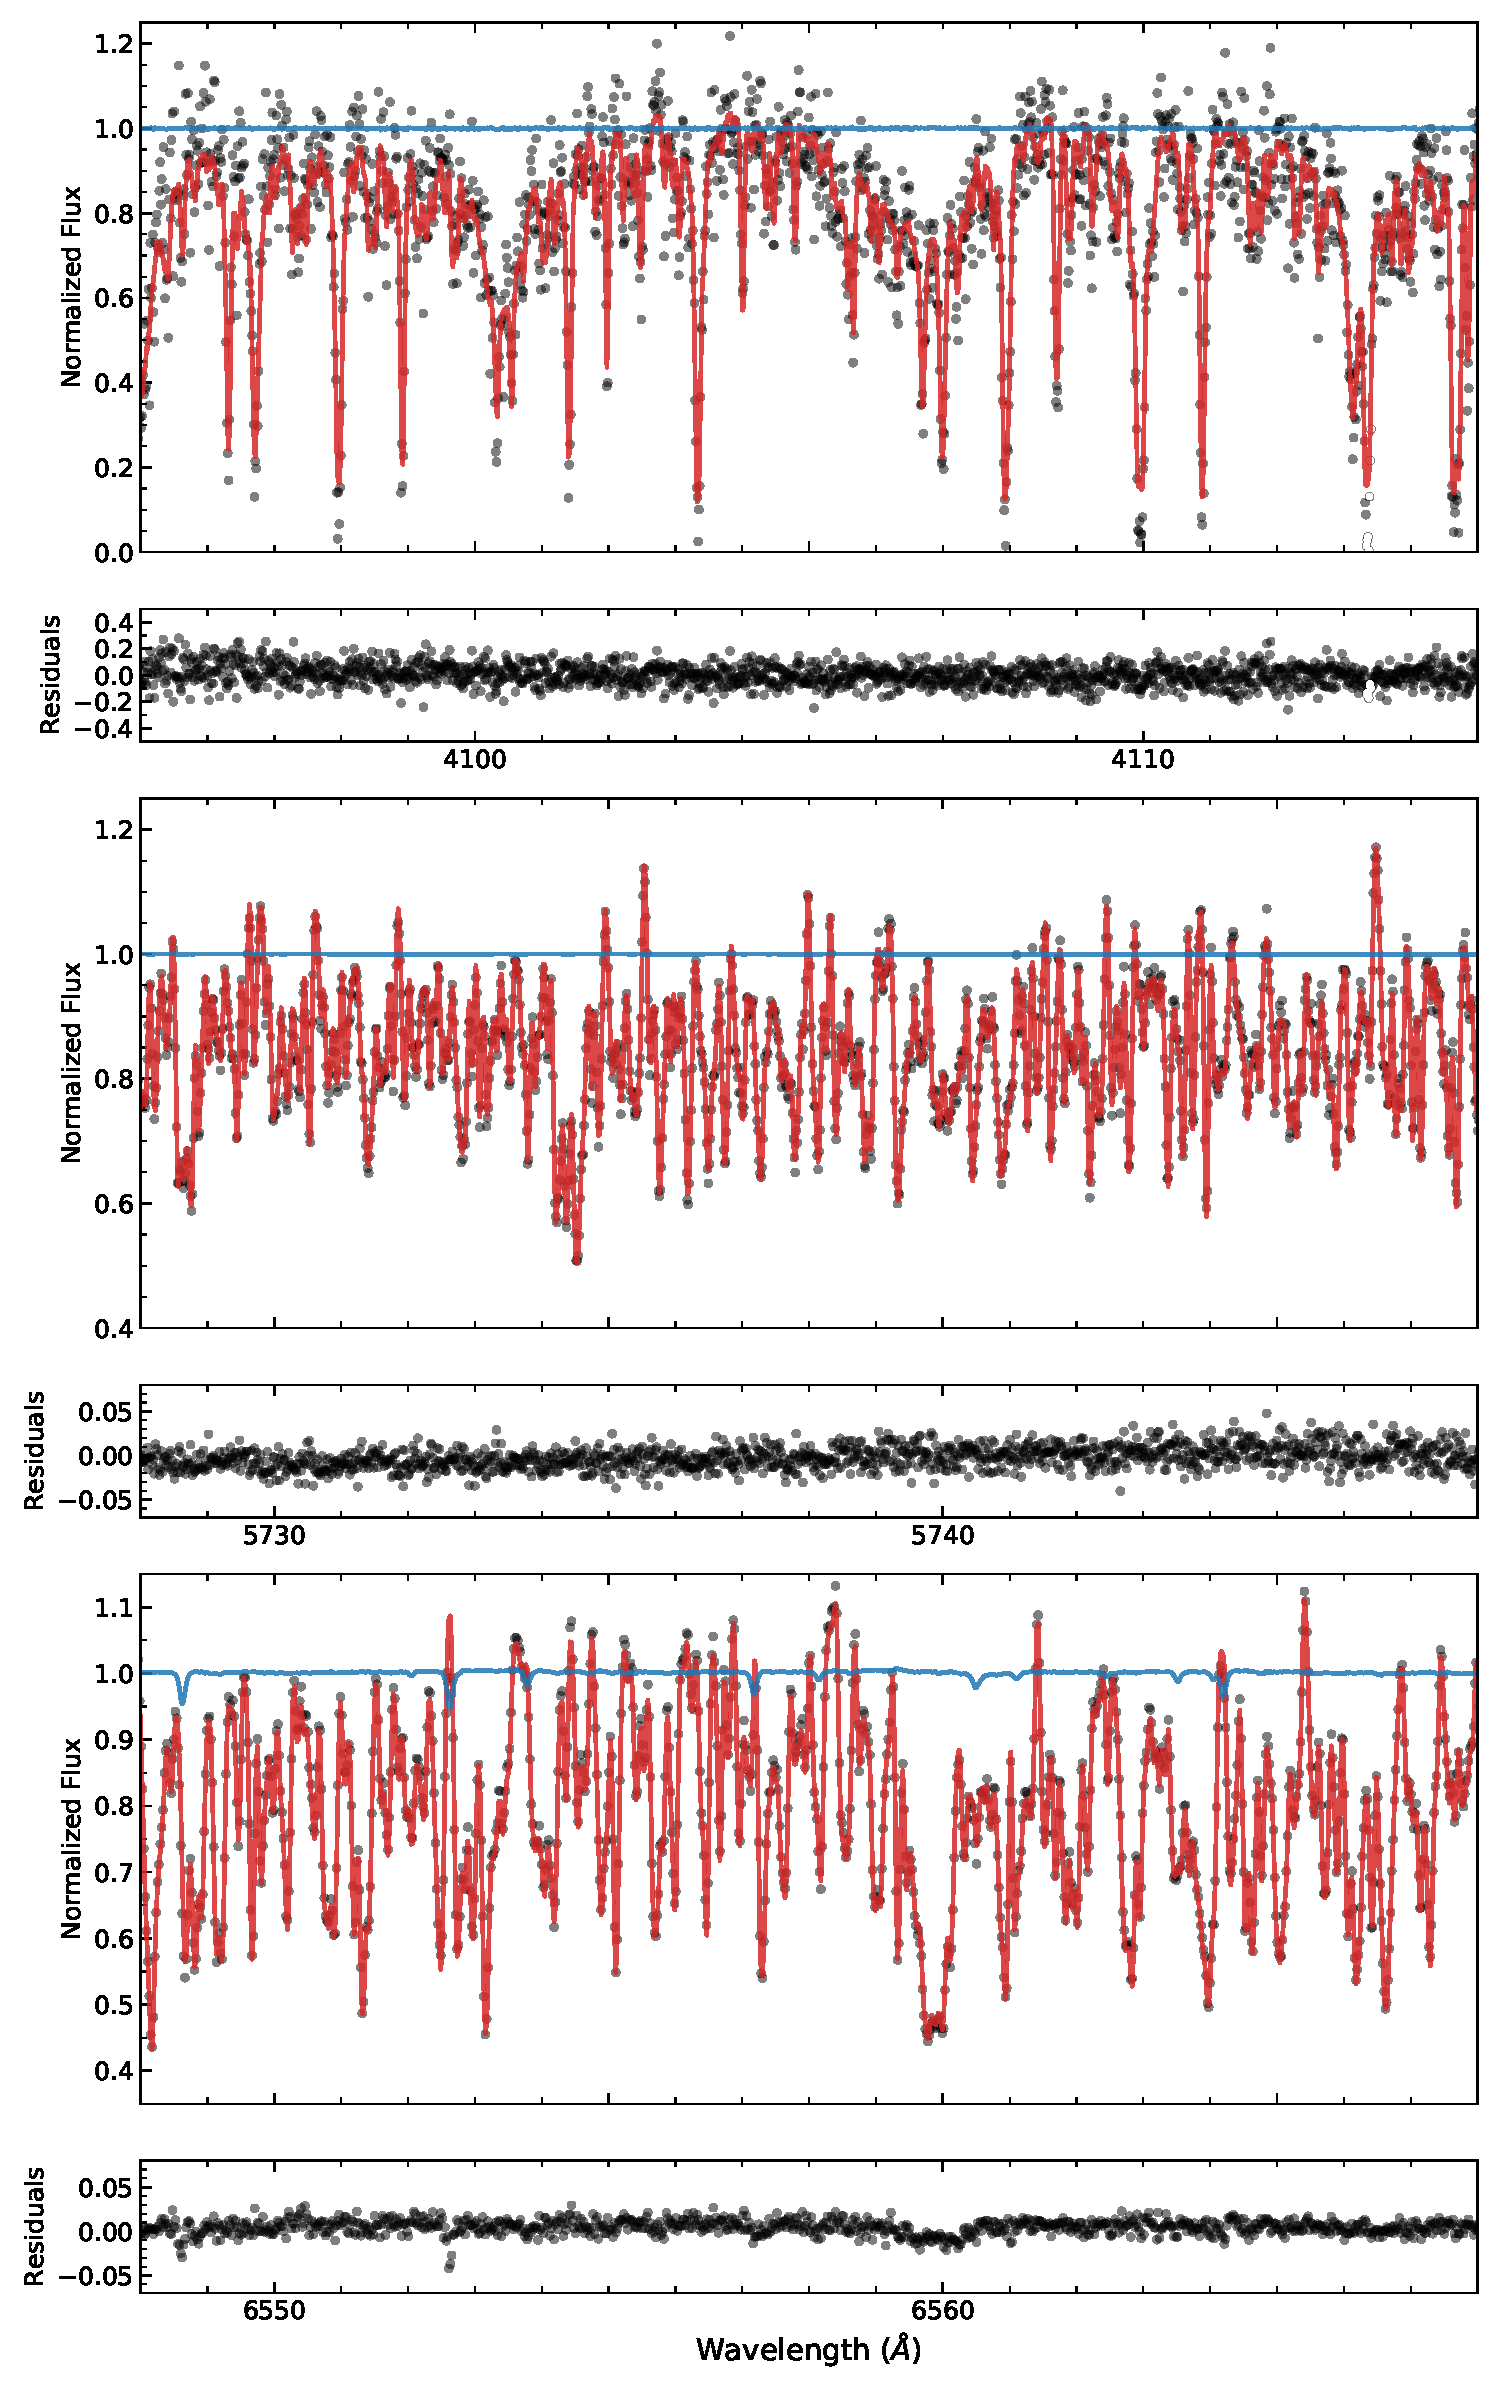
\includegraphics[width=5.5in]{barnards_multispectrum}
\caption{Example echelle orders at a randomly chosen epoch from the \HARPS observations of Barnard's Star, plotted as in Figure \ref{fig:51peg_spectrum}. \todo{(to do: weaken telluric regularization to try and get missing line at 6576 \ang)}}
\label{fig:barnards_spectrum}
\end{figure}

\begin{figure}
\centering
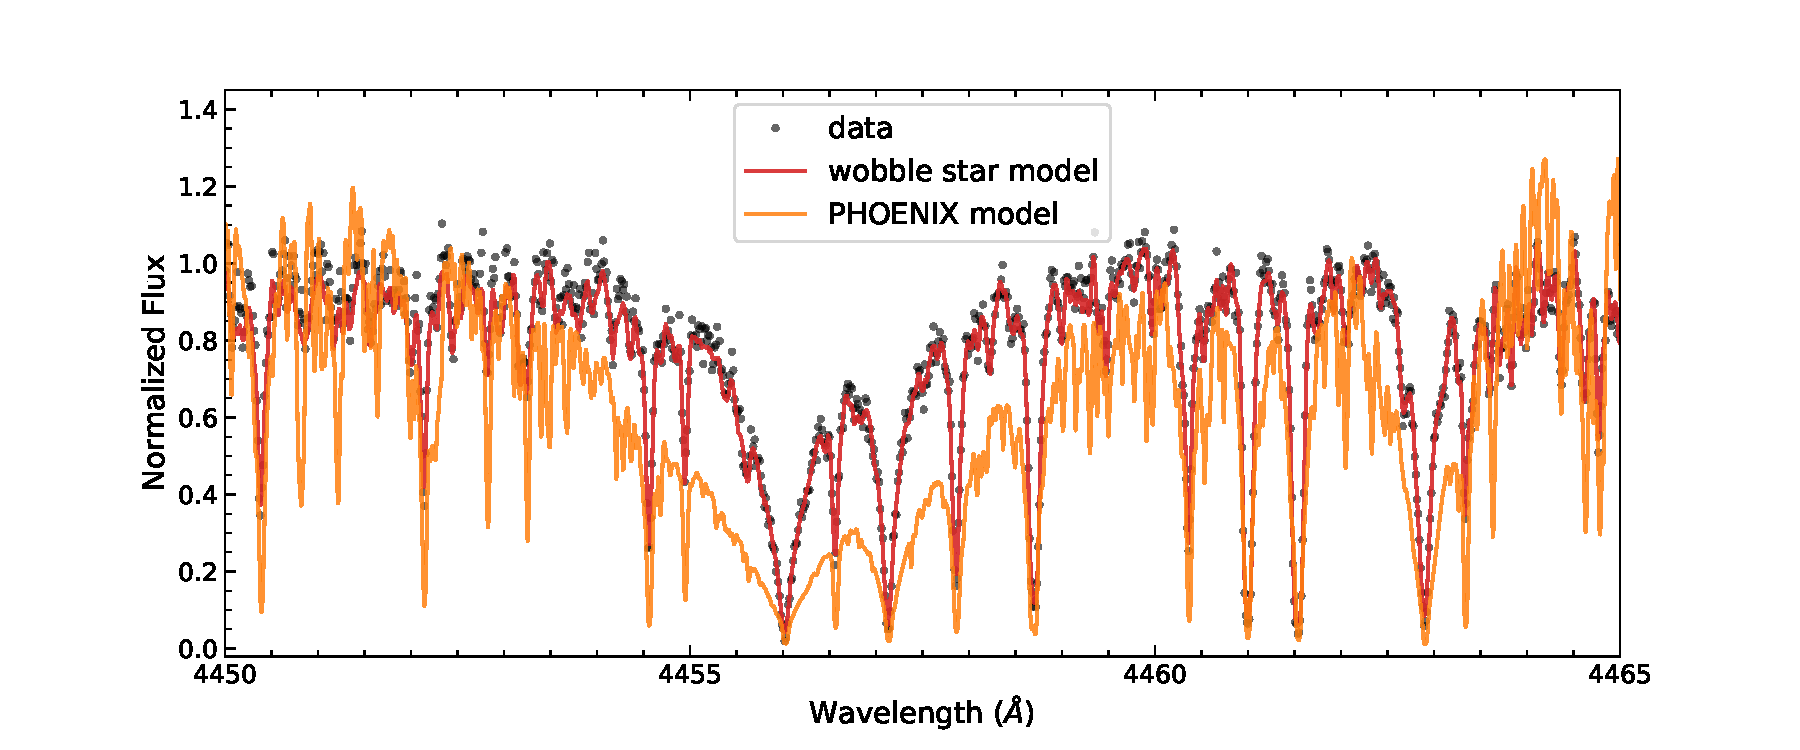
\includegraphics[width=6in]{barnards_model}
\caption{A subset of the \Mdwarf spectrum including the sodium doublet at 4456-7 \ang. The spectral template derived by \wobble is shown as a red line, while a theoretical \PHOENIX model for an M dwarf with \teff = 3200 K, \logg = 5.0, and \mh = $-0.5$ is shown as a blue line. The \wobble model has been Doppler-shifted to match the rest-frame line positions.}
\label{fig:barnards_model}
\end{figure}

One consequence of working in the low-\SNR regime is that the power to resolve very small telluric features is reduced. 
To keep the template spectra from overfitting the noise, the regularization amplitudes on the templates must be raised by several orders of magnitude relative to what was optimal for the 51 Peg fit above, particularly in orders where no strong spectral features are available. 
This has the side effect of flattening out weak features if no strong lines are present in a given order. 
As a result, we are able to retrieve fewer telluric lines in the bluer orders (compare the top panels of Figures \ref{fig:51peg_spectrum} and \ref{fig:barnards_spectrum} \todo{-- To do: check if there's a better example order}). 
In redder orders, where the \SNR is higher and more strong telluric lines are present, the features are retrieved (bottom panel of Figure \ref{fig:barnards_spectrum}). 
However, telluric variability was not able to be resolved in the overwhelming majority of orders \todo{(check on this and whether RVs are affected by K setting)}. 
We therefore caution that difficult-to-resolve microtellurics and time-variable features may not be reliably disentangled from the stellar spectrum when \wobble is applied to lower signal observations \todo{(\SNR $\lessapprox 100$ pixel$^{-1}$)}.

Despite the extreme noise at the bluer end of the wavelength range, where \Mdwarf is very faint, \wobble successfully retrieves a template spectrum that appears consistent with general expectations for a mid-M dwarf through most of the \HARPS wavelength range. 
As a sanity check, we compare the \wobble stellar template model with a high-resolution \PHOENIX model at \Mdwarf's previously measured spectral parameters \citep[\teff = 3200 K, \logg = 5.0, and \mh = $-0.5$;][and references therein]{Husser2013, Artigau2018}. 
Even in the bluest regions, the features inferred by \wobble compare well with the \PHOENIX predictions in broad strokes (Figure \ref{fig:barnards_model}). 
\todo{(check in about opacity binning affecting the smaller features)} 

These results emphasize the potential value of \wobble data products for spectral characterization and model testing, particularly in the case of faint stars and M dwarfs, for which many spectra must be combined to get a reasonably detailed composite spectrum. 
The \wobble algorithm is a simple yet robust method for doing such multi-spectra stacking while preserving telluric-contaminated regions and marginalizing over unknown \RV shifts.

\subsection{HD 189733}

\begin{figure}
\centering
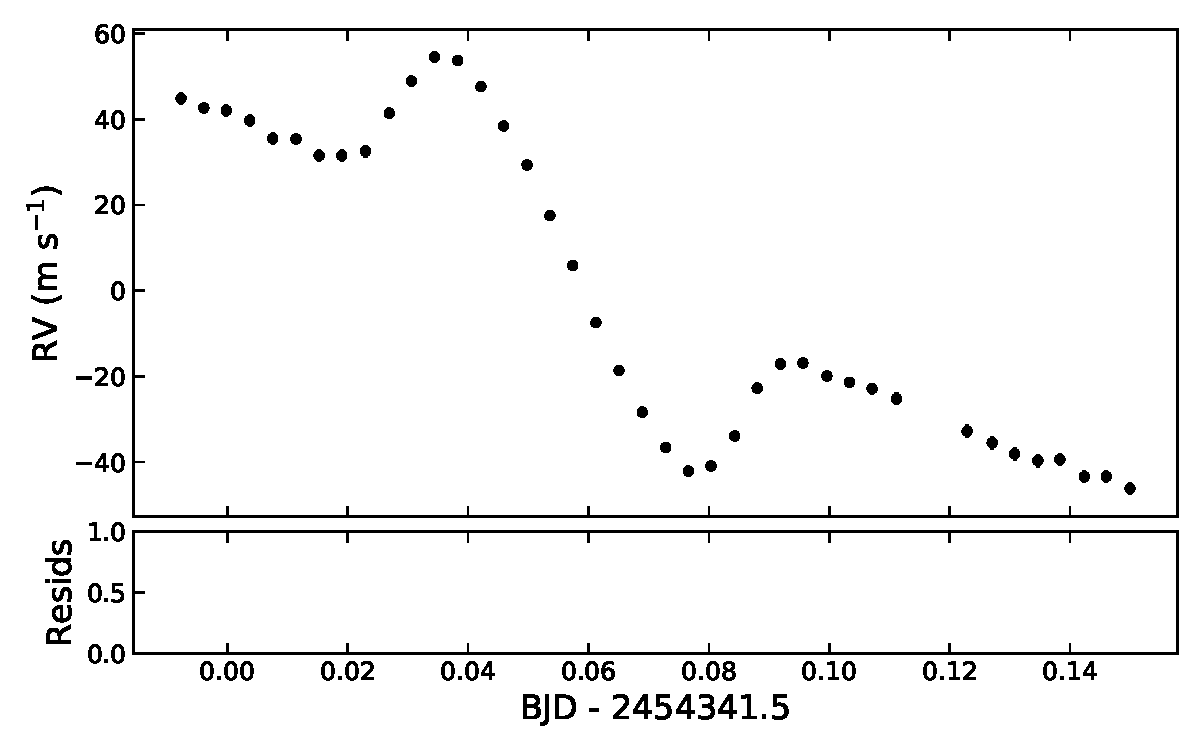
\includegraphics[width=5in]{hd189_rm}
\caption{\RVs measured by \wobble for a single night of observations of the Hot Jupiter host HD 189733. The \RM is clearly seen as the planet transits the star. \todo{[blah blah starry blah]}}
\label{fig:hd189_rm}
\end{figure}

While the majority of \EPRV measurements are made for the purposes of observing stellar reflex motion due to planetary orbits, several other applications to exoplanet characterization exist for such high-precision time-series spectra. 
One of these uses is measuring the \RM, in which the apparent stellar \RV is observed during planetary transit as a way of mapping the stellar surface and learning the spin-orbit inclination of the system \citep[e.g.][]{Queloz2000, Winn2005}. 
While the \RM technically manifests in the stellar spectrum as a distortion to the line profile rather than a true Doppler shift, it is typically detected using similar methods to a standard \RV analysis. 

We apply \wobble to a data set consisting of a single transit of the hot Jupiter HD 189733b to test its sensitivity to stellar line asymmetries as well as its performance in the regime of a single night's observations. 
The observations in question consist of a consecutive series of 40 spectra, each with an \SNR $\sim 90$, taken on the night of August 28, 2007.\footnote{Based on data obtained from the ESO Science Archive Facility under request numbers \todo{x}.} 

Because all observations came from a single night, there will be no significant shift of the stellar spectrum with respect to the telluric spectrum and the power of \wobble to disentangle the two is severely limited. 
For this reason, we fixed the telluric spectrum to a constant template. 
We derived this template by running \wobble on the 51 Peg data with non-time-variable tellurics and adopting the resulting high-quality time-invariant telluric spectrum. 
The stellar spectrum of HD 189733 and its \RVs were left as free parameters.

The resulting \RV signal retrieved by \wobble is shown in Figure \ref{fig:hd189_rm}. 
We fit the signal using \starry \citep{Luger2018}. \todo{(TO DO: fill in with Rodrigo)} 
\todo{(comparison of retrieved parameters to previous work here)} 

These results confirm that the \wobble method measures line asymmetries as \RV shifts in the same manner as traditional \RV analysis techniques. 
While this is a useful approximation in the case of the \RM, in general the confusion of these two spectral changes is a major cause of correlated noise in \RV time series \citep[e.g.][]{}. 
The simplicity and extensibility of the \wobble method is useful in this regard, as the model could be modified in a relatively straightforward manner to fit line asymmetries and true Doppler shifts separately. 
This would help to disentangle signals caused by photospheric features like starspots from the \RV signal due to reflex motion in a planetary system. 
We discuss this prospect further in Section \ref{s:future}.


\section{Telluric Features}
\label{s:tellurics}

In the above analyses, telluric spectra were inferred independently for the 51 Peg and \Mdwarf data sets. 
However, in principle the telluric features should be common to all \HARPS spectra, an assumption that we used for the case of HD 189733. 

We show a comparison between 51 Peg and \Mdwarf telluric fits in Figure \ref{fig:telluric_comparison}. 
Although they were fit using entirely different data sets with dissimilar stellar spectra, the resulting telluric fits are indeed extremely similar. 
This is generally true for all wavelength regions in which tellurics are detected. 
The only regime in which the comparison fails is for low-\SNR spectral orders of the \Mdwarf data, where the telluric spectra are featureless due to the strong regularization, as discussed in Section \ref{s:Mdwarf}. 

The physically motivated expectation that all observations should share a common telluric component could be built into the \wobble model. 
For the fit to HD 189733, for example, we fixed the telluric spectrum to use the model inferred from the better-studied star 51 Peg. 
A more robust, albeit more computationally expensive, approach would be to fit many stars simultaneously so that their shared telluric spectrum can be inferred using all the available data. 
Given enough spectra, this approach should yield an incredibly detailed model of telluric features and their time variability. 
We leave such an effort to future work. 

As another test of our derived telluric spectra, we compared the mean template from 51 Peg to an observation of the telluric standard star \todo{HR 3090 (+details)}.\footnote{Based on data obtained from the ESO Science Archive Facility under request numbers mbedell:385782 and } 
As shown in Figure \ref{fig:telluric_standard}, the spectra agree well. 
Moreover, the composite telluric spectrum inferred from the time series of 51 Peg observations is at a much higher \SNR than the single shot telluric standard spectrum, so that low-amplitude lines which border on statistical insignificance in the standard star show up clearly in the \wobble results. 
Unlike a traditional telluric standard observation, no overhead time is required to produce these results.

Of course, one strength of a telluric standard star is that its spectrum can capture the true telluric spectrum at any given moment in time, while the telluric template determined by \wobble is time-averaged and may not perfectly capture the telluric absorption lines in any given observation. 
For this reason, we included time-variable components in the model. 
A physical interpretation of these components should be possible.

An example of the inferred variability from the 51 Peg analysis is shown in Figure \ref{fig:telluric_basis}. 
There is clearly coherent structure in the variations. 
As we might expect, many of the lines co-vary with each other: as all known telluric lines in this region arise from H$_2$O, this likely corresponds to time-variable levels of atmospheric water vapor content. 
In general, the basis vectors are suggestive of Doppler shifts, perhaps due to wind speeds in different layers of the atmosphere contributing individually to the overall line shapes. 
These hypotheses could be tested in the future by seeking correlations between basis weights and externally-measured weather diagnostics. 
\todo{(is this enough? also show that basis weights change seasonally-ish?)}

\begin{figure}
\centering
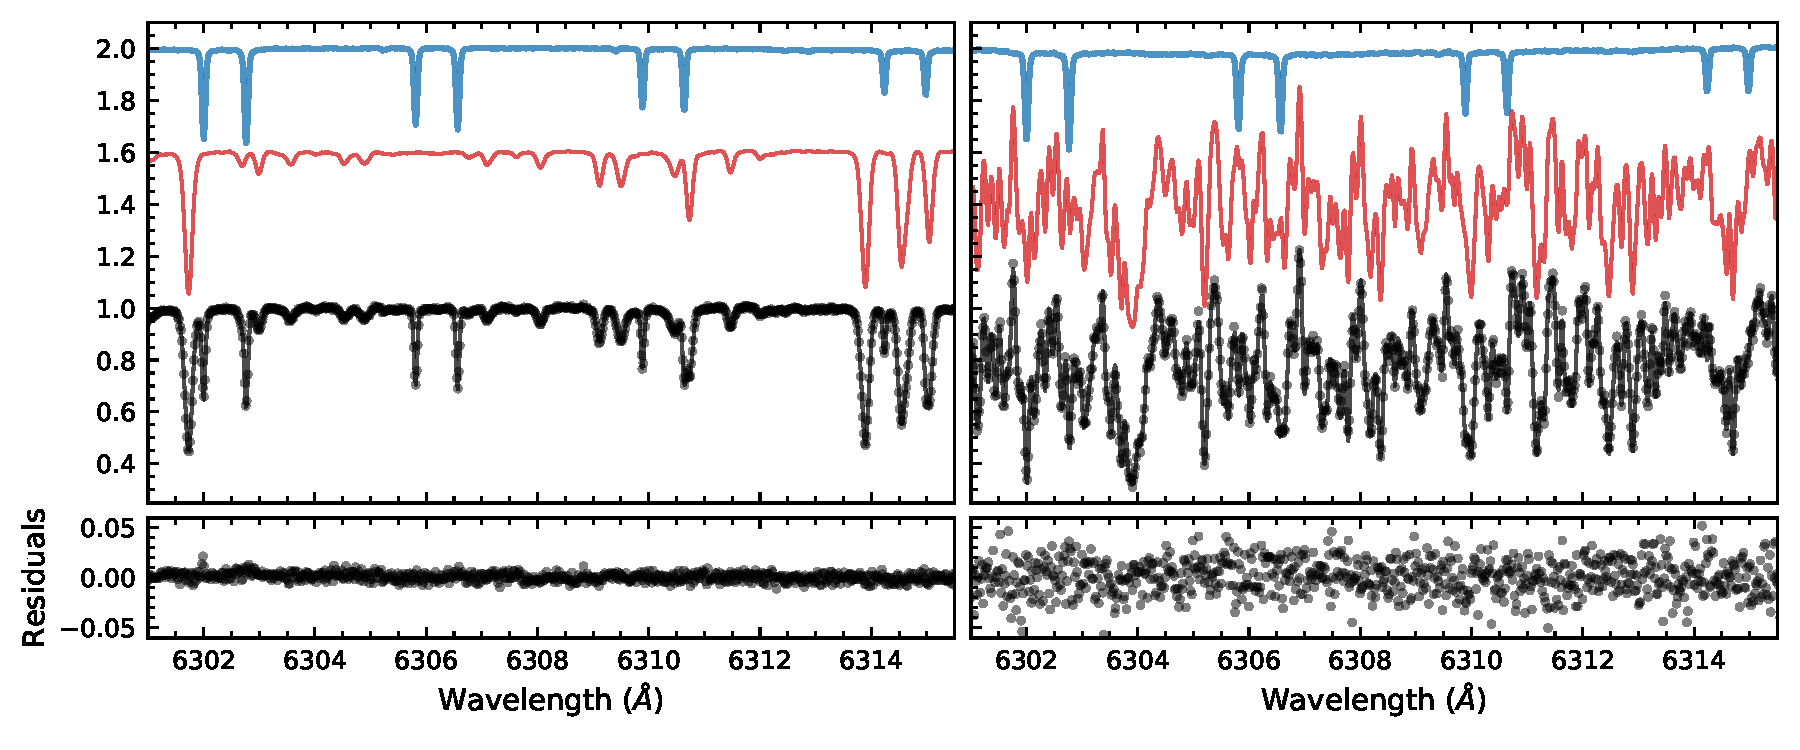
\includegraphics[width=6.5in]{telluric_comparison}
\caption{Fits to a 15-\ang region with substantial telluric contamination for 51 Peg (left) and \Mdwarf (right). The upper panels show the \wobble best-fit telluric spectrum (blue line), best-fit stellar spectrum (red line), data (black points), and the sum of the telluric and stellar model predictions (black line). Residuals are shown in the lower panels. Although the fits to each data set were performed entirely independently, the optimized telluric spectra are nearly identical, demonstrating that \wobble successfully finds an accurate representation of the common telluric absorption spectrum.}
\label{fig:telluric_comparison}
\end{figure}

\begin{figure}
\centering
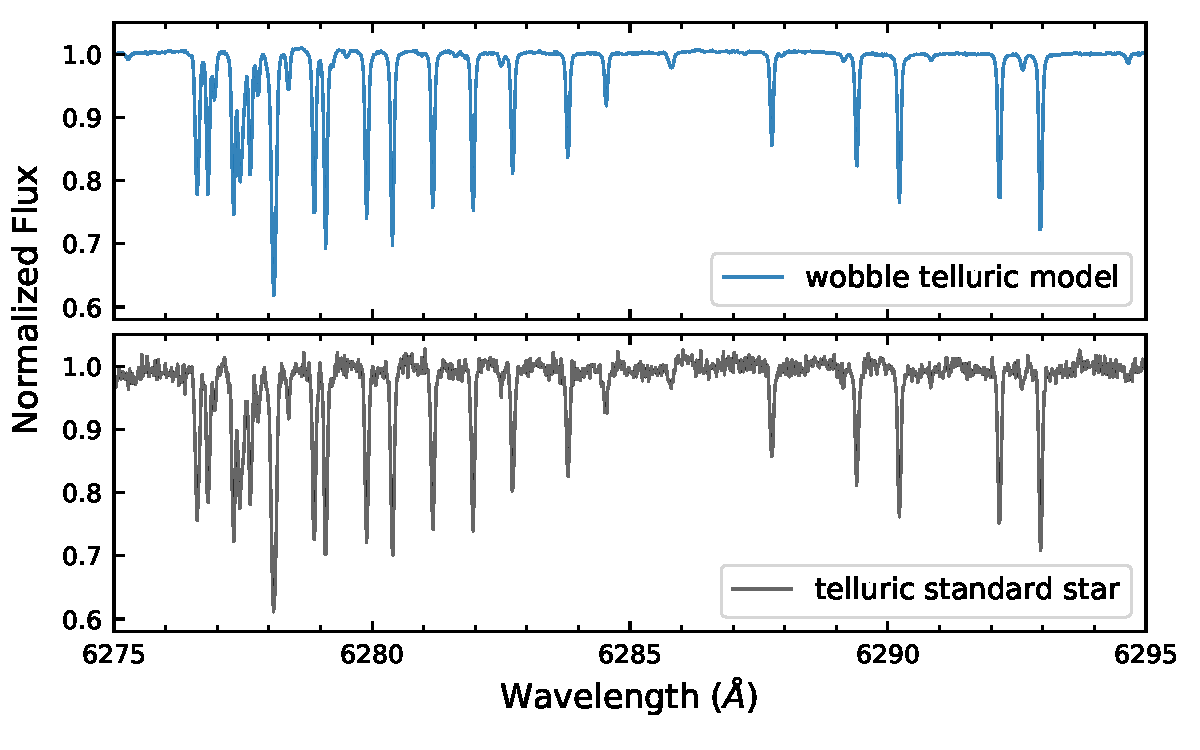
\includegraphics[width=5in]{telluric_standard}
\caption{Comparison of telluric spectrum derived by \wobble analysis of 51 Peg spectra (upper panel) and the spectrum observed with a telluric standard star (lower panel) around an H$_2$O absorption band. The \wobble method delivers a very high \SNR telluric spectrum with no overhead observing time required.}
\label{fig:telluric_standard}
\end{figure}

\begin{figure}
\centering
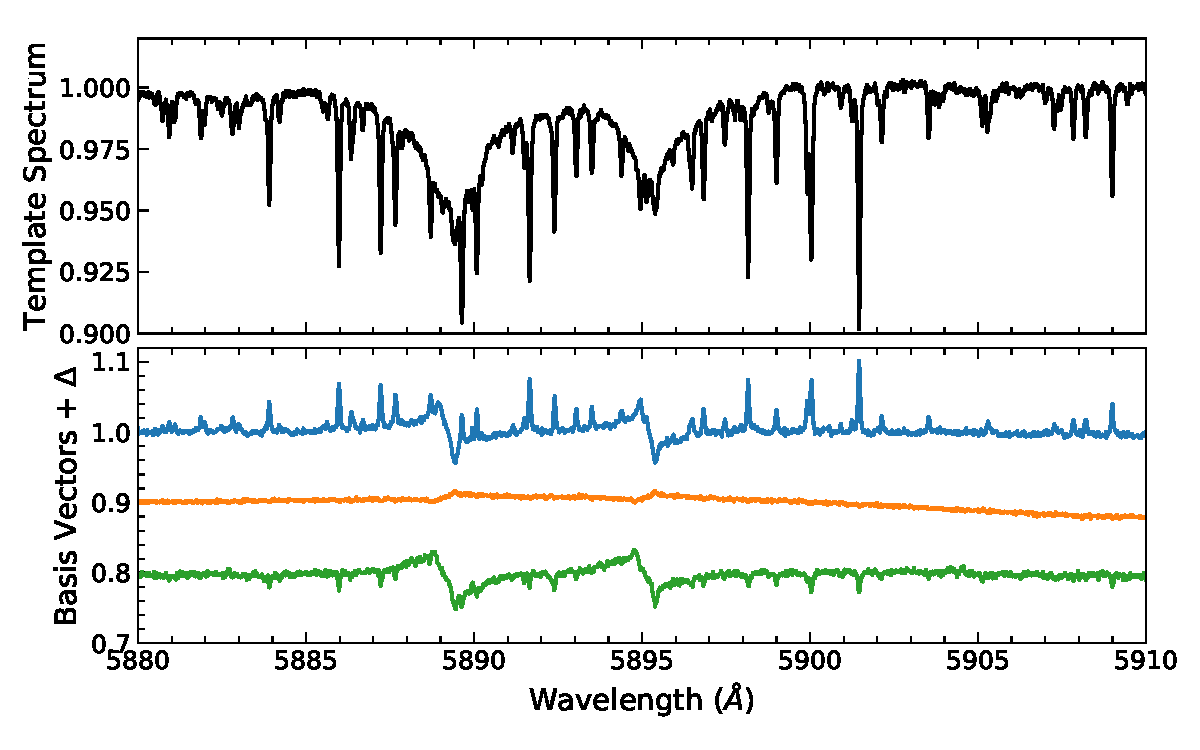
\includegraphics[width=5in]{telluric_basis2}
\caption{Example of the mean telluric spectral template in a small wavelength region (upper panel) and the three basis vectors used to capture the time-variable contributions to the spectrum, staggered by an arbitrary offset for display (lower panel).}
\label{fig:telluric_basis}
\end{figure}

\section{Limitations and Extensibility of \wobble}
\label{s:future}

In this work we have tested \wobble exclusively using \HARPS data, but vast amounts of data from other \EPRV instruments exist and may benefit from the techniques used here. 
We now turn our discussion to ways in which other data sets may violate the assumptions made in this work and the corresponding modifications to \wobble that would enable it to operate more effectively in these regimes. 
For simplicity, we break this discussion down into three categories: inherent limitations of \wobble; assumptions that could be eliminated; and general changes that may improve the \RV precision achieved by \wobble.

\subsection{Inherent Limitations}

limitations on number of spectra: Experiment with sub-sampling 51 Peg to fewer epochs. \wobble does have many free parameters and therefore it's not going to work well for very few epochs. Also telluric sampling is key. in some regime \wobble is just not the right tool for the job.

low-SNR limitations: what we did is a hack and it should be possible to do much better with better continuum normalization. but still you'll eventually hit a failure mode.

spectrograph resolution: will this work if lines are undersampled?

\subsection{Revisiting Assumptions}

single star: this actually isn't a true assumption, it's trivial to add an extra star, or even a planetary component, to the model.

no gas cell: should be as simple as adding an extra component (Of course, gas cells exist because calibration isn't perfect...)

reliable instrument calibration: use tellurics to modify wavelength calibration? (there are relevant citations here) Spectral variability due to LSF changing? Additional parameters to the P operators, non-convex optimization

low-dimensional telluric variability: it's possible this isn't true in the current parameterization. what if we work with residuals away from a physical model of the tellurics? or reparameterize lines 

constant stellar spectrum: cite \citet{Davis2017} for PCA approach. Some absorption lines are more sensitive to the effects of stellar activity than others (Dumusque). If these fall into a small number of categories, a PCA-like dimensionality reduction should do well. Address pros and cons of introducing Gaussian processes to parameterize line profiles. deal with this similarly to the LSF changing? also, maybe we need to regularize (or put priors on) the \RVs themselves and force them to sum of Keplerians for the purpose of breaking degeneracies with stellar variability.

\subsection{General Improvements}

\begin{itemize}

\item Regularization framework could be improved: we chose it because it is convex and represents our beliefs but it's the most difficult and unwieldy part of \wobble.

\item Spectral representation: ours sucks. Could go to higher-order interpolation scheme like cubic split OR smooth non-parametric rep like a GP OR something that incorporates more physics. Nothing about wobble depends on the spectral representation and it should be simple to swap out for something better provided it can be implemented in \TF.

\item Spectral continuum!!! All methods are questionable at low SNR and in the absence of true continuum. Right solution is to simultaneously fit continuum with other model components, but this introduces degeneracies and must be handled carefully.

\item We treat the orders separately: we mostly did this to break up the computation, but this could be changed straightforwardly. Doing so would take on additional computational cost, but we are in \TF so it shouldn't hurt too much.

\item We could fit all stars simultaneously, which would give a much better telluric template

\item 1D extracted spectra. Our P operators are interpolators onto 1D data but they could be 2D interpolators! Little about the model equations would change, but implementation would become much trickier.

\end{itemize}

\section{Conclusion}
\label{s:conclusion}

Extracting precise \RVs is important and will become more critical as new instruments come online. 

Fundamental data-driven technique - requires no physics knowledge which makes it a great tool for expanding \RV searches.  
Open-source, can be adapted for use with any current or future \EPRV instrument
...

Here's what this enables. 

\todo{[TO DO: add software citations]}

\acknowledgements{It is a pleasure to acknowledge Jacob L. Bean, Heather Knutson, Timothy Morton, Melissa Ness, Hans-Walter Rix, Andreas Seifahrt, and Julian St\"{u}rmer for helpful discussions. 

This research has made use of the services of the ESO Science Archive Facility. 

This work has made use of data from the European Space Agency (ESA) mission
{\it Gaia} (\url{https://www.cosmos.esa.int/gaia}), processed by the {\it Gaia}
Data Processing and Analysis Consortium (DPAC,
\url{https://www.cosmos.esa.int/web/gaia/dpac/consortium}). Funding for the DPAC
has been provided by national institutions, in particular the institutions
participating in the {\it Gaia} Multilateral Agreement.}

\bibliographystyle{apj}
\bibliography{paper.bib}%general,myref,inprep}

\end{document}  